\clearpage
\SourceLeaf{605}\pdfbookmark[0]{Manuscript Papers.}{handschriftlicher-nachlass}
\thispagestyle{empty}
\vspace*{35mm}
\begin{center}
{\large MANUSCRIPT}\par\vspace{20mm}
{\LARGE PAPERS.}
\end{center}
\clearpage
\SourceLeaf{607}\fancyhead[L]{\small MANUSCRIPT PAPERS.}
\pdfbookmark[1]{On the Mathematical Theory of Electrodynamic Effects.}{electrodynamische-wirkungen}
\begin{center}
{\large ON THE MATHEMATICAL THEORY}\par\vspace{3mm}
{\large OF ELECTRODYNAMIC EFFECTS.}
\end{center}
\begin{center}[1.]\end{center}
The general fundamental law for the \textit{intensity in the individual parts of a galvanic current system} can be reduced to the following conception.

It is enough to consider wires of equal thickness, since differences in thickness can be accounted for by using different numbers of wires. For example, if a wire were of thickness $=2$ in one part and $=3$ in another, one could substitute the system
\begin{center}\resizebox{.62\linewidth}{!}{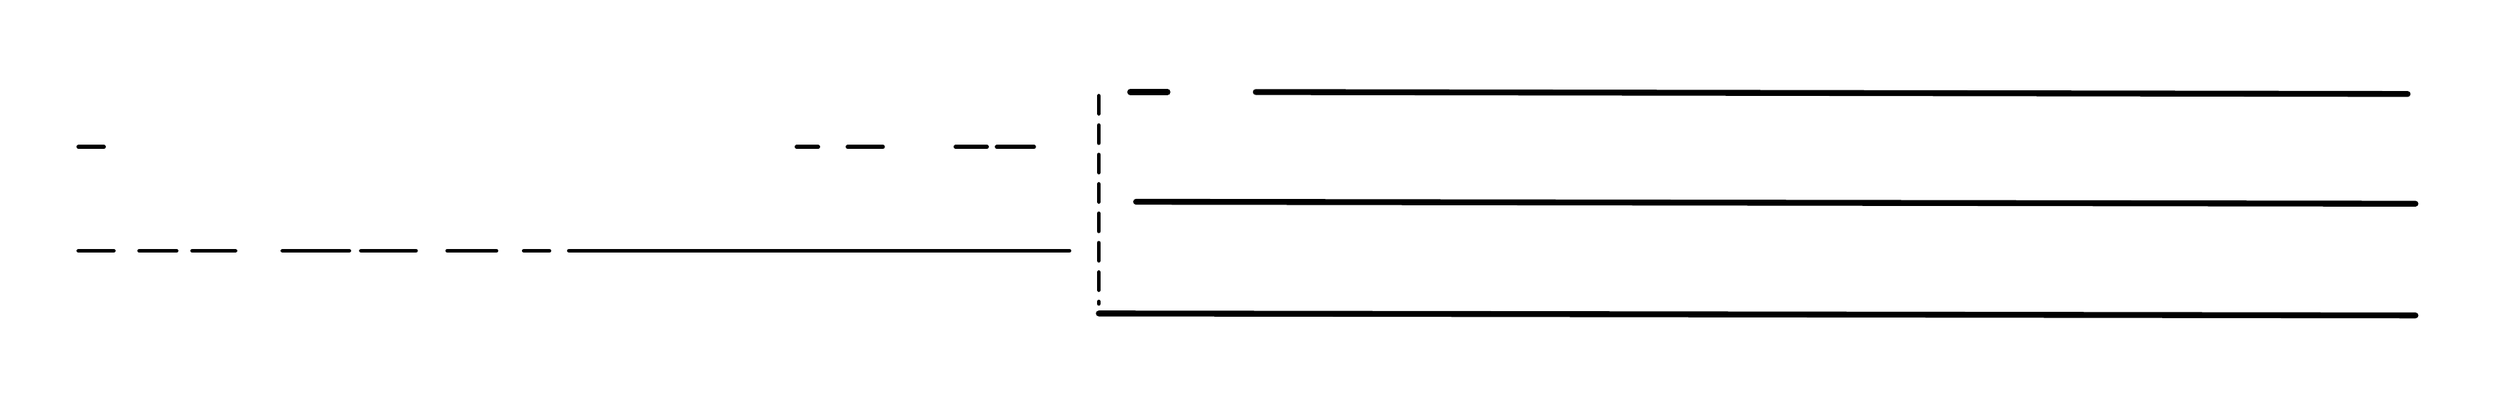
\begin{tikzpicture}[x=1bp,y=-1bp,line cap=round,line join=round]
\path[use as bounding box] (0,0) rectangle (1254,184);
\begin{pgfinterruptboundingbox}
\draw[line width=2bp] (30,65) -- (43,65);
\draw[line width=2bp] (396,65) -- (407,65);
\draw[line width=2bp] (422,65) -- (440,65);
\draw[line width=2bp] (477,65) -- (493,65);
\draw[line width=2bp] (498,65) -- (517,65);
\draw[line width=2bp] (30,118) -- (48,118);
\draw[line width=2bp] (61,118) -- (80,118);
\draw[line width=2bp] (88,118) -- (110,118);
\draw[line width=2bp] (134,118) -- (168,118);
\draw[line width=2bp] (174,118) -- (202,118);
\draw[line width=2bp] (218,118) -- (243,118);
\draw[line width=2bp] (257,118) -- (270,118);
\draw[line width=2bp] (280,118) -- (535,118);
\draw[line width=3bp] (566,37) -- (585,37);
\draw[line width=3bp] (630,37) -- (1217,38);
\draw[line width=3bp] (569,93) -- (1221,94);
\draw[line width=3bp] (550,150) -- (1221,151);
\draw[line width=2.1bp,dash pattern=on 9bp off 6bp] (550,39) -- (550,145);
\end{pgfinterruptboundingbox}
\end{tikzpicture}
}\end{center}
shown here.

The question, then, is the intensity at each point in a system of lines joined into a network like this.
\begin{center}\resizebox{.63\linewidth}{!}{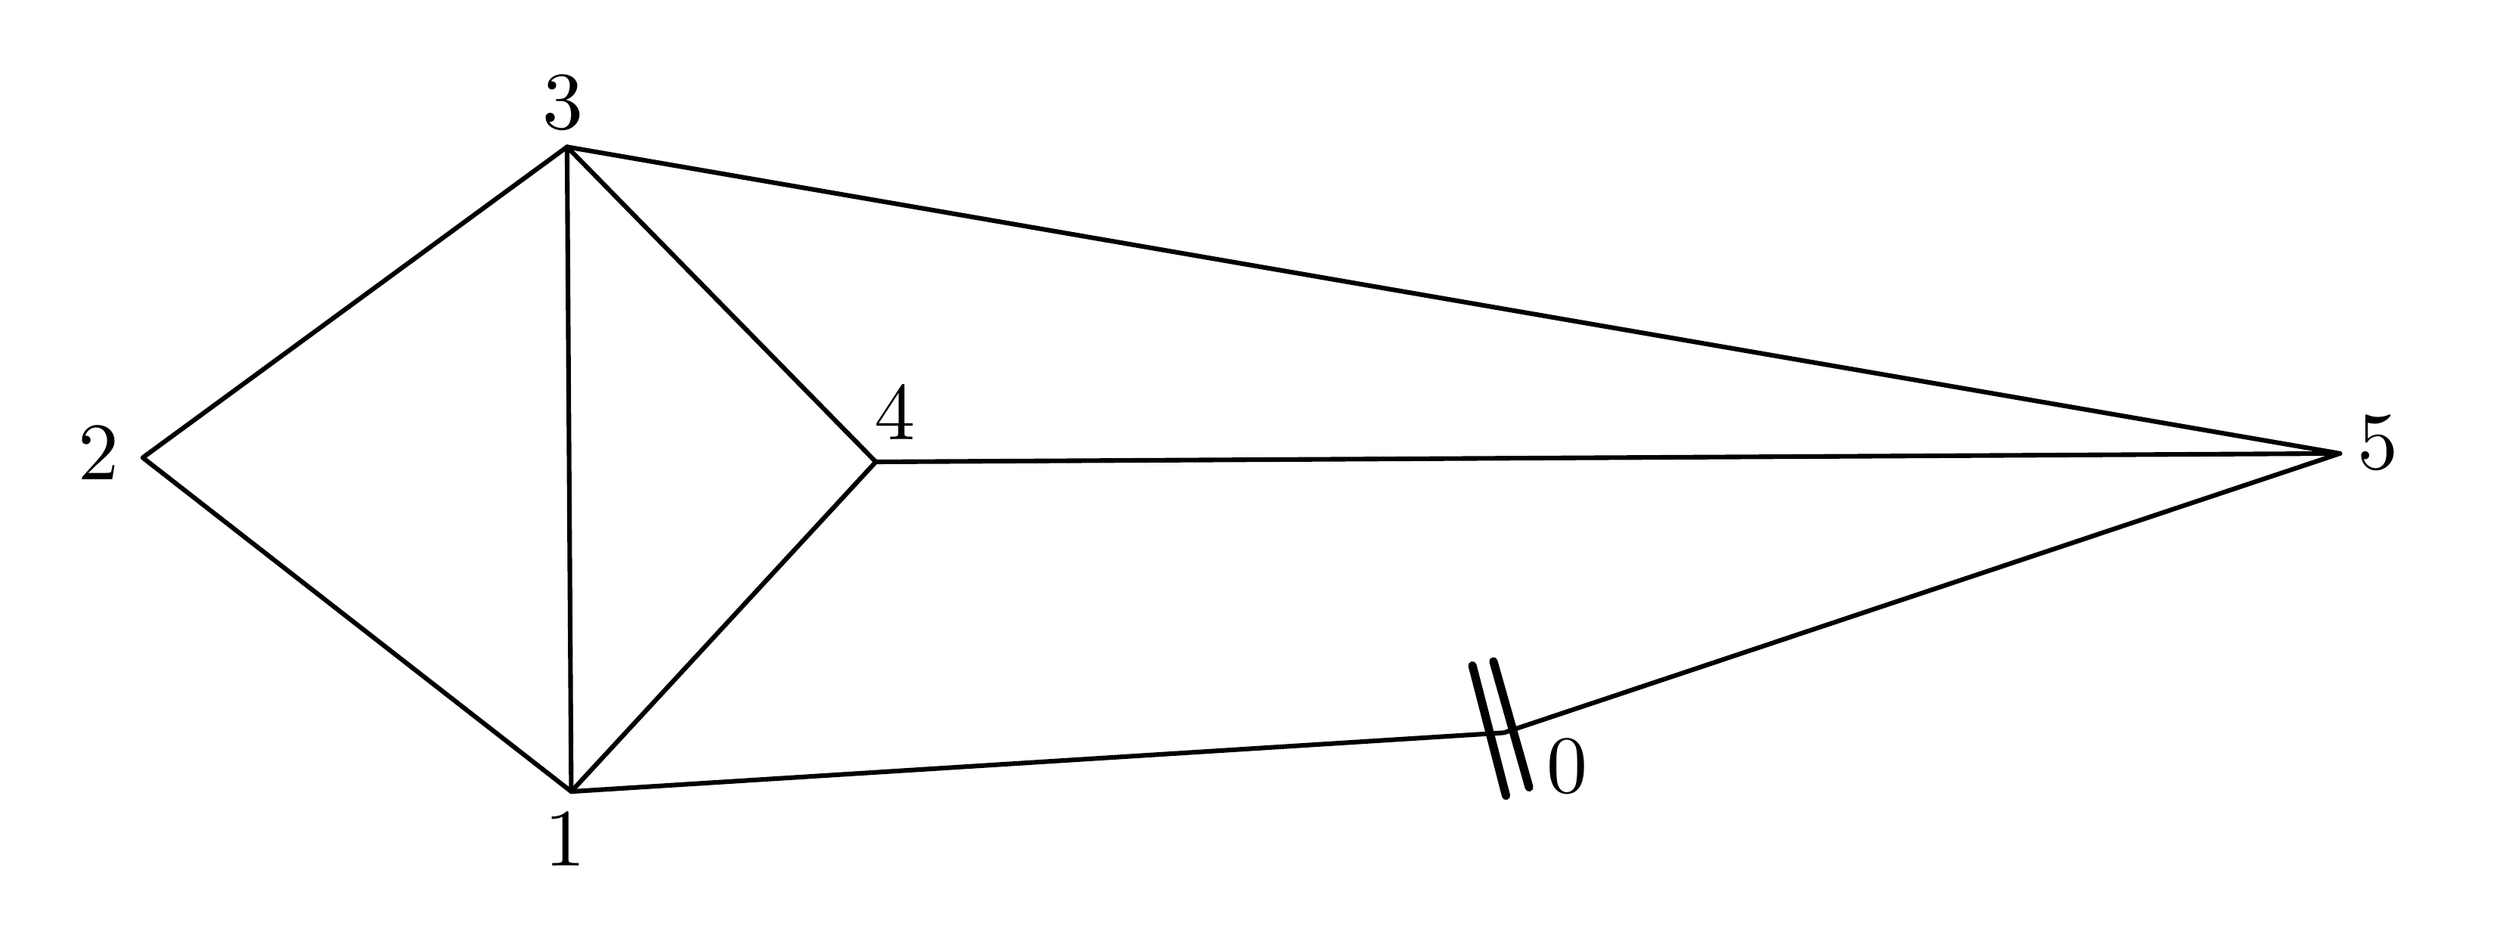
\begin{tikzpicture}[x=1bp,y=-1bp,line cap=round,line join=round]
\path[use as bounding box] (0,0) rectangle (1170,421);
\begin{pgfinterruptboundingbox}
\draw[line width=2.2bp] (262,367) -- (58,208) -- (260,60) -- (407,210) -- (262,367);
\draw[line width=2.2bp] (260,60) -- (262,367);
\draw[line width=2.2bp] (260,60) -- (1104,206) -- (407,210);
\draw[line width=2.2bp] (262,367) -- (706,339) -- (1104,206);
\draw[line width=4bp] (691,307) -- (707,369);
\draw[line width=4bp] (701,305) -- (718,365);
\node[inner sep=0pt,outer sep=0pt] at (259,390) {\scalebox{3.9}{\ensuremath{1}}};
\node[inner sep=0pt,outer sep=0pt] at (37,206) {\scalebox{3.9}{\ensuremath{2}}};
\node[inner sep=0pt,outer sep=0pt] at (258,39) {\scalebox{3.9}{\ensuremath{3}}};
\node[inner sep=0pt,outer sep=0pt] at (416,187) {\scalebox{3.9}{\ensuremath{4}}};
\node[inner sep=0pt,outer sep=0pt] at (1122,201) {\scalebox{3.9}{\ensuremath{5}}};
\node[inner sep=0pt,outer sep=0pt] at (736,355) {\scalebox{3.9}{\ensuremath{0}}};
\end{pgfinterruptboundingbox}
\end{tikzpicture}
}\end{center}
In place of all these locations, one need consider only the points where more than 2 lines meet and the seats of force. At each point in the system the intensity has \textit{one} value, and at the seats of force it has \textit{two}.

\SourceLeaf{608}The general fundamental law is as follows. Suppose $A$ is an arbitrary point, $A',\ A'',\ A'''\,.\,.$ are points each joined to $A$ by a simple connection, and there is no point $B$ for which $AB$ is part of none of $AA',\ AA'',\ AA'''\,.\,.$ and contains none of them. For each point one must then assume something analogous to a height, with $a$ at point $A$, $a'$ at point $A'$, and so on. Then the following always holds
\[
0=\frac{a'-a}{AA'}+\frac{a''-a}{AA''}+\frac{a'''-a}{AA'''}+\,.\,.
\]
and the individual terms of this sum always express the current intensity in the individual parts.

\vspace{3mm}
The general solution to the preceding problem is as follows. Let $A^0,\ A^{n+1}$ be the two poles, $A',\ A'',\ A'''$ etc.\ $A^n$ the individual junctions of the system, and $\frac{1}{f^{\alpha,\beta}}$ the total resistance along the simple path from $A^\alpha$ to $A^\beta$. The denominator is thus to be set $=0$ when there is no direct connection between the points. Determine from the equations
\[
\begin{aligned}
(f^{1,0}+f^{1,2}+f^{1,3}+\,.\,.)p'-f^{1,0}p^0-f^{1,2}p''-f^{1,3}p'''-\text{etc.}&=0\\
(f^{2,0}+f^{2,1}+f^{2,3}+\,.\,.)p''-f^{2,0}p^0-f^{2,1}p'-f^{2,3}p'''-\text{etc.}&=0\\
(f^{3,0}+f^{3,1}+f^{3,2}+\,.\,.)p'''-f^{3,0}p^0-f^{3,1}p'-f^{3,2}p''-\text{etc.}&=0
\end{aligned}
\]
and so on,\quad together with the following
\[
p^0\ \text{arbitrary},\quad p^{n+1}=p^0+k,\quad k\ \text{denoting the generating force},
\]
the quantities $p',p'',p'''\,.\,.$. The strength of the current between $A^\alpha$ and $A^\beta$ is then
\[
=f^{\alpha,\beta}(p^\beta-p^\alpha)
\]

\vspace{3mm}
The fundamental principle can be stated even more simply as follows.

At every point there is a \textit{definite} pressure as soon as its value at \textit{one} point has been chosen arbitrarily. Two statements then suffice to express everything in equations.

I.\quad Let $A,\ B$ be two points with no junction between them, $P$ the sum of the forces between these points reckoned in the direction from $A$ to $B$, $\rho$ the total resistance between them, and $a,\ b$ the pressure values at those points. Then $\frac{a-b+P}{\rho}=$ the intensity of the current in the direction from $A$ to $B$.

\SourceLeaf{609}II.\quad The sum of the intensities of all the currents reckoned outward from one point (more than two at a junction) is $=0$.

\begin{center}[2.]\end{center}
In the diagram, let $a,b,c,d,e,f$ be the resistances in the marked sections, with the source of the current in $a$. Further, let
\begin{center}\resizebox{.28\linewidth}{!}{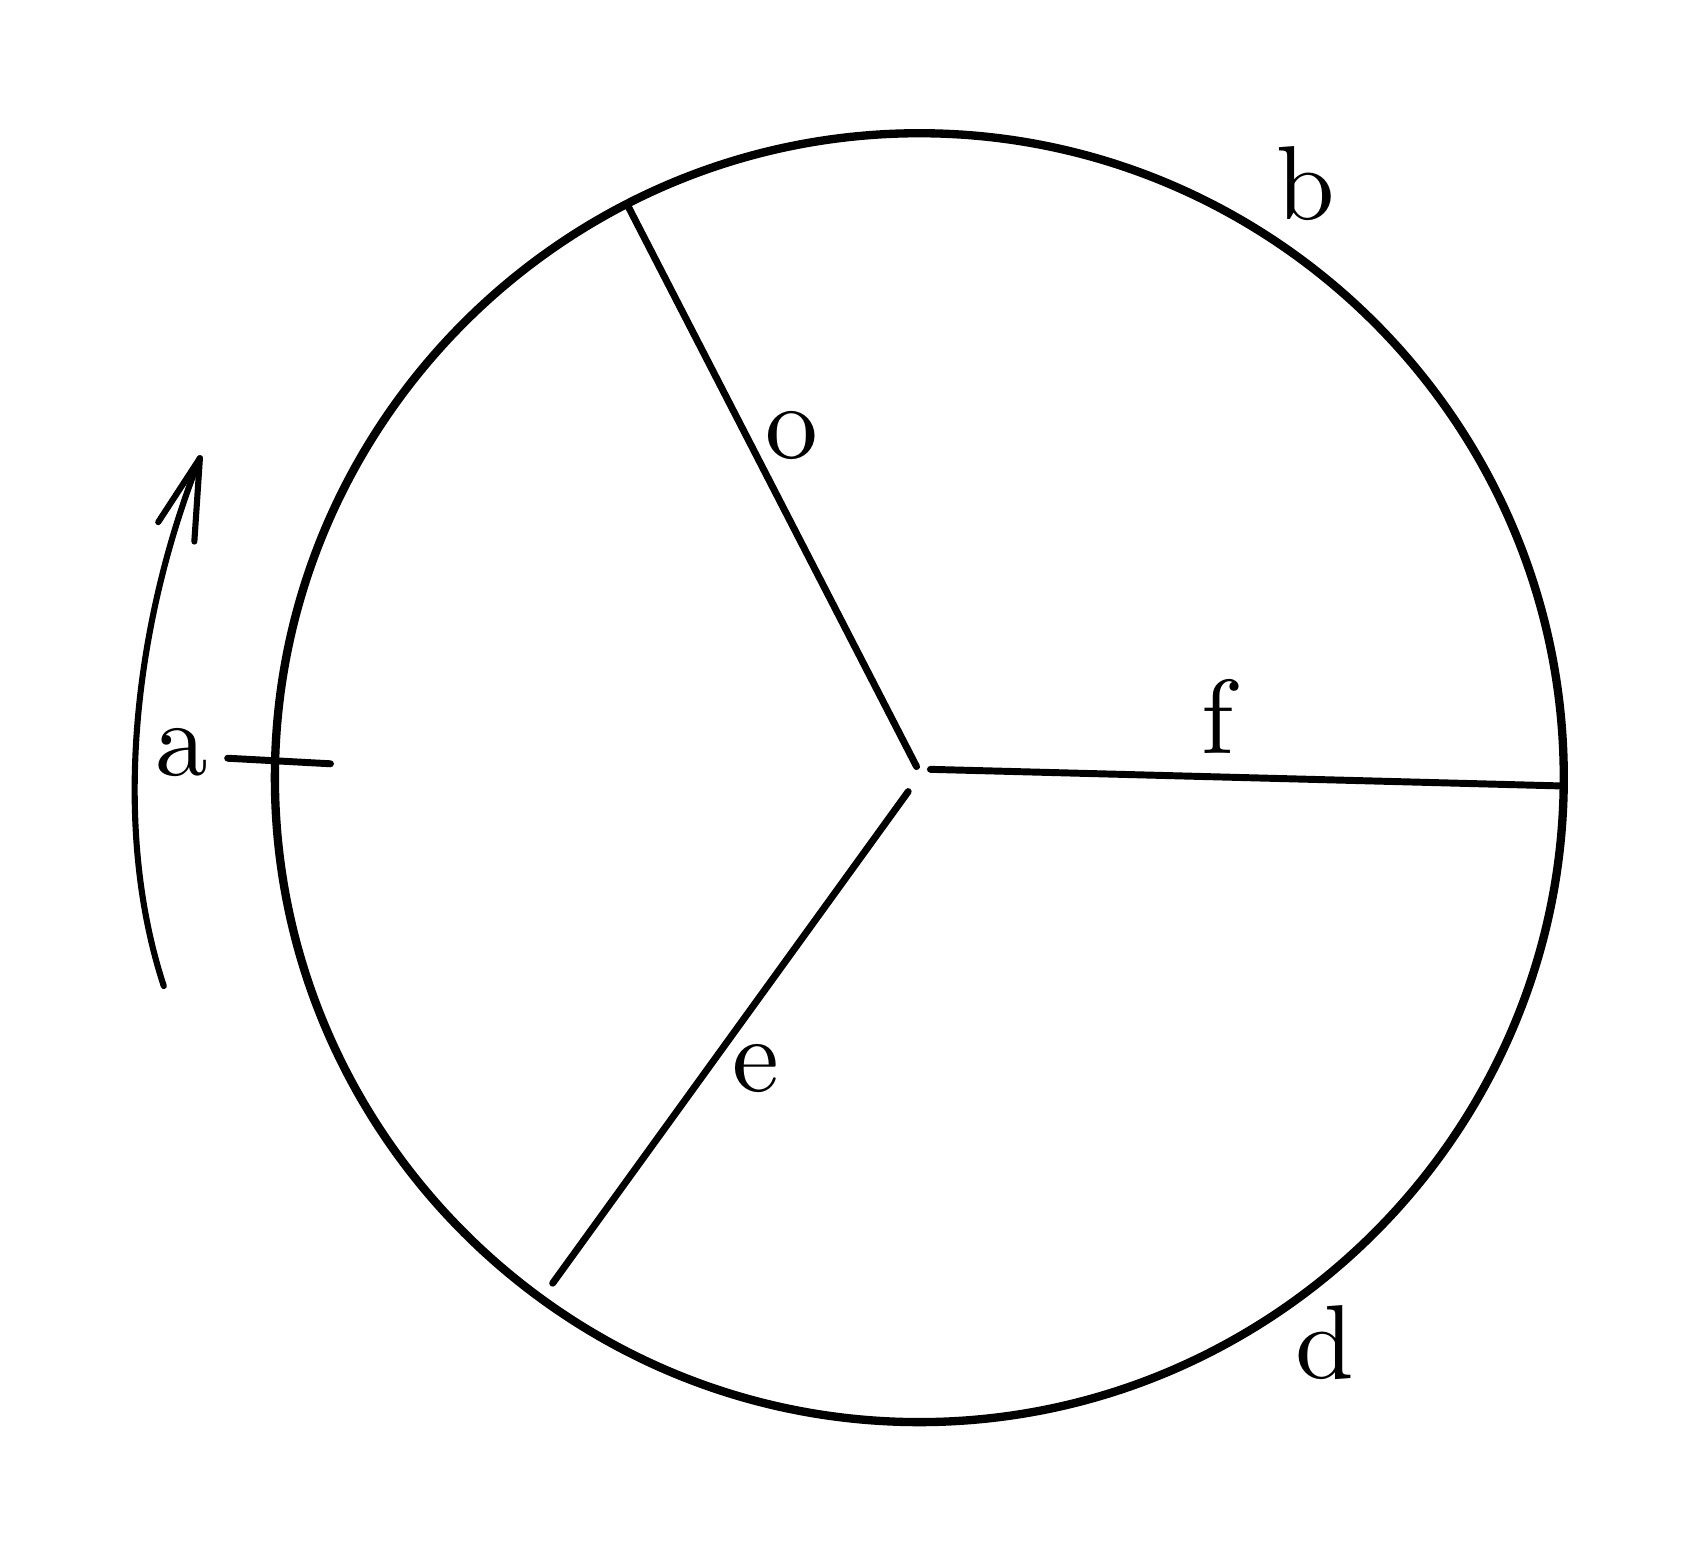
\begin{tikzpicture}[x=1bp,y=-1bp,line cap=round,line join=round]
\path[use as bounding box] (0,0) rectangle (588,535);
\begin{pgfinterruptboundingbox}
\draw[line width=3bp] (321,38) .. controls (448.60,38) and (553,142.40) .. (553,270) .. controls (553,397.60) and (448.60,502) .. (321,502) .. controls (193.40,502) and (89,397.60) .. (89,270) .. controls (89,142.40) and (193.40,38) .. (321,38);
\draw[line width=2.5bp] (216,64) -- (320,266);
\draw[line width=2.5bp] (325,267) -- (553,273);
\draw[line width=2.5bp] (317,275) -- (189,452);
\draw[line width=2.5bp] (72,263) -- (109,265);
\draw[line width=2.2bp] (49,345) .. controls (29,284) and (40,210) .. (62,155);
\draw[line width=2.2bp] (47,178) -- (62,155) -- (60,185);
\node[inner sep=0pt,outer sep=0pt] at (55,261) {\scalebox{3.8}{\ensuremath{\mathrm{a}}}};
\node[inner sep=0pt,outer sep=0pt] at (460,56) {\scalebox{3.8}{\ensuremath{\mathrm{b}}}};
\node[inner sep=0pt,outer sep=0pt] at (275,147) {\scalebox{3.8}{\ensuremath{\mathrm{o}}}};
\node[inner sep=0pt,outer sep=0pt] at (467,473) {\scalebox{3.8}{\ensuremath{\mathrm{d}}}};
\node[inner sep=0pt,outer sep=0pt] at (262,375) {\scalebox{3.8}{\ensuremath{\mathrm{e}}}};
\node[inner sep=0pt,outer sep=0pt] at (430,248) {\scalebox{3.8}{\ensuremath{\mathrm{f}}}};
\end{pgfinterruptboundingbox}
\end{tikzpicture}
}\end{center}
\[
\begin{aligned}
(b+c)(d+e)+f(b+d+c+e)&=p\\
bcde\left(\frac{1}{b}+\frac{1}{c}+\frac{1}{d}+\frac{1}{e}\right)+f(b+d)(c+e)&=q
\end{aligned}
\]
Then the total resistance of the system without section $a$
\[
=\frac{q}{p}
\]
and the intensity is
\[
\begin{aligned}
A&=\frac{(b+c)(d+e)+f(b+c+d+e)}{ap+q}=\frac{p}{ap+q}\\[4pt]
B&=\frac{cd+ce+cf+ef}{ap+q}\\[4pt]
C&=\frac{bd+be+bf+df}{ap+q}\\[4pt]
D&=\frac{be+ce+cf+ef}{ap+q}\\[4pt]
E&=\frac{bd+cd+bf+df}{ap+q}\\[4pt]
F&=\frac{be-cd}{ap+q}
\end{aligned}
\]
The fundamental principle also leads to the conclusion that
\[
\sum rii
\]
must be a minimum, where $r$ denotes the resistance corresponding to an element and $i$ the intensity of the current. More simply still,
\[
\sum\varepsilon vv
\]
must attain a minimum, where $\varepsilon$ denotes an element of the moving fluid and $v$ the velocity.

\SourceLeaf{610}If 0, 1, 2, etc. are the junctions in a network of conductors, with
\begin{center}\begin{tabular}{rl}
$r^{01}$ & the resistance\\
$i^{01}$ & the strength of the current from 0 to 1\\
$p^{01}$ & the motive force from 0 to 1 in the connecting section 01\\
$q^0$ & the pressure at 0\quad and so on, then
\end{tabular}\end{center}
\[
\begin{aligned}
\text{I.}\quad q'-q^0&=p^{01}-i^{01}r^{01}\\
\text{II.}\quad 0&=i^{01}+i^{02}+i^{03}+\text{etc.}
\end{aligned}
\]
From this, if all the $p$ and $r$ are given, all the $q$ and $i$ can be determined.

Let $\Omega=\sum pi$ over all combinations. Since it follows from II that
\[
\sum(q'-q^0)i^{01}=0
\]
one obtains
\[
\Omega=\sum iir
\]
If one considers a second system of values in which the $p$ remain unchanged and the $r$ change by an infinitesimal amount, then
\[
\begin{aligned}
\mathrm d\Omega&=\sum ii\,\mathrm dr+2\sum ir\,\mathrm di=-\sum ii\,\mathrm dr+2\sum i\,.\,\mathrm dir\\
&=-\sum ii\,\mathrm dr-2\sum i^{01}(\mathrm dq'-\mathrm dq^0)=-\sum ii\,\mathrm dr
\end{aligned}
\]
Thus any decrease in one $r$, with the others unchanged, increases $\Omega$.

\begin{center}[3.]\end{center}
The action of \textit{two galvanic current elements} 0, 1 \textit{on each other}, according to my conception, which, incidentally, still needs further examination, is as follows.

Let the coordinates of the two current elements be $x,y,z$ and $x',y',z'$, distance $=r$. For the current elements themselves, $\mathrm dx=\xi$, $\mathrm dy=\eta$, $\mathrm dz=\zeta$, $\mathrm dx'=\xi'$, etc. For the action experienced by the second, $\delta\xi'=X'$, $\delta\eta'=Y'$, etc. Then
\[
\begin{aligned}
r^3X'&=\xi\{(y'-y)\eta'+(z'-z)\zeta'\}-(x'-x)(\eta\eta'+\zeta\zeta')\\
r^3Y'&=\eta\{(z'-z)\zeta'+(x'-x)\xi'\}-(y'-y)(\zeta\zeta'+\xi\xi')\\
r^3Z'&=\zeta\{(x'-x)\xi'+(y'-y)\eta'\}-(z'-z)(\xi\xi'+\eta\eta')
\end{aligned}
\]

